%###########################################################################
%
% Anhang
%
%###########################################################################
%\begin{appendix}
%\label{chap:Appendix}
%\chapter{Appendix A}
%\setcounter{chapter}{1}
%\addcontentsline{toc}{chapter}{Appendix}
%###########################################################################
% Anhang A
%###########################################################################
%\label{A}
%....


%\chapter{Appendix B}
%###########################################################################
% Anhang B
%###########################################################################
%\label{B}

%\pagebreak
%###########################################################################
%\end{appendix}

\renewcommand\thesection{\Alph{section}}
\renewcommand\thefigure{\thesection\arabic{figure}}
\renewcommand{\thetable}{\thesection\arabic{table}}
\setcounter{figure}{0}
\setcounter{table}{0}
\setcounter{section}{0}

\chapter*{Appendix}
\addcontentsline{toc}{chapter}{Appendix}

\label{chap:Appendix}

\section{Radiation}
\label{sec:AppendixRadiation}

All calculations and figures in \autoref{sec:AppendixRadiation} are performed with SPENVIS unless otherwise stated.

%TODO welche Tools verwendet und welchen Orbit zum simulieren
%TODO letzte Schicht Si

\begin{figure}[htb]
     \centering
     \begin{subfigure}[b]{0.49\textwidth}
         \centering
         \includegraphics[width=\textwidth]{Media/E_Electron_Flux}
         \caption{Average spectra of trapped electrons around Earth}
         \label{fig:trappedelectronsEarth}
     \end{subfigure}
     \hfill
     \begin{subfigure}[b]{0.49\textwidth}
         \centering
         \includegraphics[width=\textwidth]{Media/E_Proton_Flux}
         \caption{Average spectra of trapped protons around Earth}
         \label{fig:trappedprotonsEarth}
     \end{subfigure}
     \hfill
     \begin{subfigure}[b]{0.49\textwidth}
         \centering
         \includegraphics[width=\textwidth]{Media/J_Electron_Flux}
         \caption{Average spectra of trapped electrons around Jupiter}
         \label{fig:trappedelectronsJupiter}
     \end{subfigure}
     \hfill
     \begin{subfigure}[b]{0.49\textwidth}
         \centering
         \includegraphics[width=\textwidth]{Media/J_Proton_Flux}
         \caption{Average spectra of trapped protons around Jupiter}
         \label{fig:trappedprotonsJupiter}
     \end{subfigure}
     \caption{Average trapped proton and electron fluxes on an orbit around earth at 25,000 km, through the outer Van Allen radiation belt, and on Europa's orbit around Jupiter.}
     \label{fig:trappedprotonelectronfluxes}
\end{figure}

\begin{figure}[htb]
     \centering
     \begin{subfigure}[b]{0.49\textwidth}
         \centering
         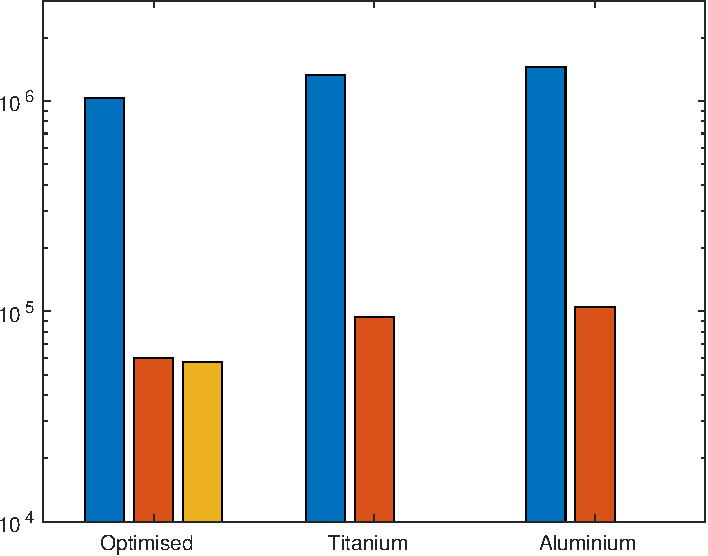
\includegraphics[width=\textwidth]{Media/J_Electron_Shielding}
         \caption{TID for Electrons as Source Particles}
         \label{fig:TIDElectronShielding}
     \end{subfigure}
     \hfill
     \begin{subfigure}[b]{0.49\textwidth}
         \centering
         \includegraphics[width=\textwidth]{Media/J_Proton_Shielding}
         \caption{TID for Proton as Source Particles}
         \label{fig:TIDProtonShielding}
     \end{subfigure}
     \caption{TID of aluminium, titanium, and the optimised radiation structure shown in \autoref{tab:OptimalRadiationProtection} with an weight target of 0.5 \(\text{g/cm}^2\) over 30 days of exposure on Europa}
     \label{fig:AluminiumTitanOptimised}
\end{figure}

\begin{table}[htb]
\centering
\caption{Material properties from Galinstan, as well as mercury and water as comparison values at 20 \textit{°C}}
\begin{adjustbox}{max width=\textwidth}
\begin{tabular}[l]{lccccc}

	\toprule
		Components	&	TID	&	Location\\
	\midrule
	
	
		&		&	 \\	
	
	
		&		&	\\
	
	
	 &		&	\\
	

	\bottomrule

\end{tabular}
\end{adjustbox}
\label{tab:RadiationList}
\end{table}

\clearpage

\section{Appendix 2}
\label{sec:Appendix2}

...

\cleardoublepage